\section{Benutzerinterface}

\subsection{Layout}
Das Layout beruht auf der gegebenen Blynk Oberfläche und einer Auswahl an verfügbaren Widgets. 

\begin{figure}[H]
    \begin{center}
    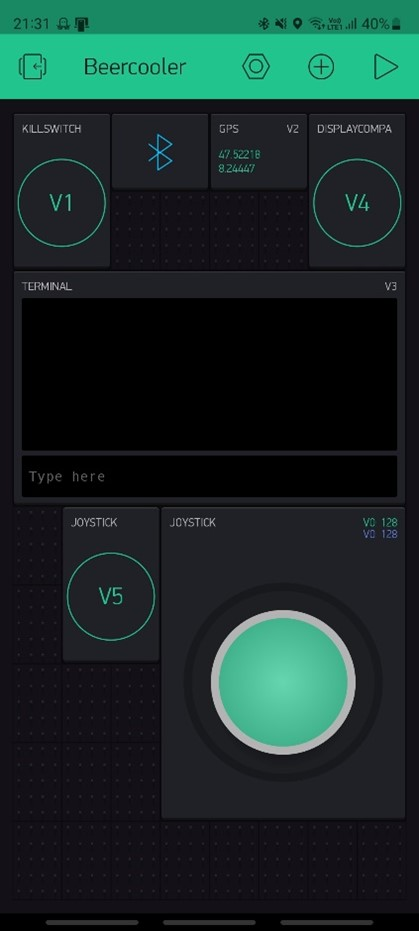
\includegraphics[width=5cm]{Layout_BlynkApp.jpg}
    \end{center}
    \caption{Layout in der Blynk App}
\end{figure}

Es soll mindestens ein Killswitch, eine Bluetooth-Verbindung, ein GPS-Stream und ein Terminal darin enthalten sein.

\subsection{Funktionen}
Über den Killswitch soll der Roboter in den “Fahren”-Modus versetzt werden können und diesen wieder verlassen. Das Bluetooth- und GPS- Widget dienen lediglich dem Informationsaustausch zwischen dem Arduino und der App. Der Terminal soll schliesslich die Möglichkeit bieten, GPS-Koordinaten direkt dem Arduino zuzuführen, zu welchen er fahren soll.